\documentclass[aspectratio=169, 10pt]{beamer}

% --- Packages ---
\usepackage[utf8]{inputenc}
\usepackage{tikz}
\usepackage{pgfplots}
\usepackage{amsmath, amssymb, amsfonts}
\usepackage{booktabs}
\usepackage{bm}
\usepackage{xcolor}
\usetikzlibrary{arrows.meta, calc, positioning, shapes.geometric, decorations.pathreplacing, backgrounds, fit, shadows, patterns, shapes.arrows, angles, quotes}
\pgfplotsset{compat=1.17}

% =============================================================================
% NYU TANDON THEME SETUP
% =============================================================================

% NYU Colors
\definecolor{nyupurple}{RGB}{87,46,140}
\definecolor{nyuheader}{RGB}{172,159,195}
\definecolor{nyufooter}{RGB}{189,178,211}

% Use default theme as base
\usetheme{default}
\setbeamertemplate{navigation symbols}{}

% Itemize colors
\setbeamercolor{itemize item}{fg=nyupurple}
\setbeamercolor{itemize subitem}{fg=nyupurple}
\setbeamercolor{itemize subsubitem}{fg=nyupurple}
\setbeamertemplate{itemize item}{\textbullet}
\setbeamertemplate{itemize subitem}{\textbullet}
\setbeamertemplate{itemize subsubitem}{\textbullet}

% Block colors
\setbeamercolor{block title}{fg=white, bg=nyupurple}
\setbeamercolor{block body}{fg=black, bg=nyuheader!30}
\setbeamercolor{block title alerted}{fg=white, bg=red!70}
\setbeamercolor{block body alerted}{fg=black, bg=red!10}
\setbeamercolor{block title example}{fg=white, bg=green!50!black}
\setbeamercolor{block body example}{fg=black, bg=green!10}

% Custom colors for diagrams
\definecolor{darkblue}{RGB}{0,51,102}
\definecolor{brightblue}{RGB}{0,102,204}
\definecolor{lightblue}{RGB}{153,204,255}
\definecolor{darkgreen}{RGB}{0,102,51}
\definecolor{accentred}{RGB}{192,0,0}
\definecolor{accentgreen}{RGB}{0,128,0}
\definecolor{accentorange}{RGB}{255,128,0}

% --- Custom Commands ---
\newcommand{\vect}[1]{\boldsymbol{#1}}
\newcommand{\mat}[1]{\mathbf{#1}}

% =============================================================================
% FRAMETITLE WITH HEADER BAR
% =============================================================================
\makeatletter
\setbeamertemplate{frametitle}{%
    \nointerlineskip%
    \begin{beamercolorbox}[wd=\paperwidth,ht=0.7cm,dp=0.15cm,rightskip=0.5cm]{frametitle}
        \hspace{0.3cm}\usebeamerfont{frametitle}\insertframetitle%
        \hfill%
        \raisebox{0.08cm}{{\bfseries\sffamily\color{nyupurple}NYU}}%
    \end{beamercolorbox}%
}
\makeatother

\setbeamercolor{frametitle}{fg=black, bg=nyuheader}
\setbeamerfont{frametitle}{size=\large}

% =============================================================================
% FOOTLINE
% =============================================================================
\setbeamertemplate{footline}{%
    \begin{tikzpicture}[remember picture, overlay]
        \fill[nyufooter] ([yshift=0.6cm]current page.south west) rectangle ([xshift=5cm]current page.south east);
        \fill[nyufooter!70] ([yshift=0.6cm, xshift=5cm]current page.south west) rectangle ([xshift=10.5cm]current page.south east);
        \fill[nyufooter!40] ([yshift=0.6cm, xshift=10.5cm]current page.south west) rectangle (current page.south east);
        
        \node[anchor=west, font=\small] at ([xshift=0.3cm, yshift=0.3cm]current page.south west) {Dr.\ Aliasghar Arab};
        \node[anchor=center, font=\small] at ([yshift=0.3cm]current page.south) {Autonomous Mobile Robots};
        \node[anchor=east, font=\small] at ([xshift=-0.3cm, yshift=0.3cm]current page.south east) {LECTURE 2 -- FALL 2025 \quad \insertframenumber{} / \inserttotalframenumber};
    \end{tikzpicture}%
}

% =============================================================================
% TITLE PAGE
% =============================================================================
\defbeamertemplate*{title page}{customized}[1][]
{
    \begin{tikzpicture}[remember picture, overlay]
        \node[anchor=north east] at ([xshift=-0.8cm, yshift=-0.8cm]current page.north east) {%
            {\bfseries\sffamily\Large\color{nyupurple}NYU}%
            {\sffamily\normalsize\color{black}\ \ TANDON SCHOOL OF ENGINEERING}%
        };
    \end{tikzpicture}
    
    \vspace{2cm}
    \centering
    {\Large\bfseries\inserttitle\par}
    \vspace{0.3cm}
    {\insertsubtitle\par}
    \vspace{1cm}
    {\insertauthor\par}
    \vspace{0.3cm}
    {\small\insertinstitute\par}
    \vspace{0.5cm}
    {\insertdate\par}
}

% =============================================================================
% TITLE INFORMATION
% =============================================================================
\title{Autonomous Mobile Robots}
\subtitle{Lecture 2: Vehicle Kinematics \& Equations of Motion}
\author{Dr.\ Aliasghar Arab}
\institute{NYU Tandon School of Engineering}
\date{Fall 2025}

% =============================================================================
% DOCUMENT
% =============================================================================
\begin{document}

% -----------------------------------------------------------------------------
% TITLE SLIDE
% -----------------------------------------------------------------------------
{
\setbeamertemplate{footline}{}
\begin{frame}[plain]
\titlepage
\end{frame}
}

% -----------------------------------------------------------------------------
% LECTURE OVERVIEW
% -----------------------------------------------------------------------------
\begin{frame}{Lecture Overview}

\textbf{\underline{Last Lecture:}} Introduction to Autonomous Mobile Robots

\vspace{0.5cm}

\textbf{\underline{This Lecture:}} Vehicle Kinematics \& Equations of Motion
\begin{itemize}
    \item Reference frames and coordinate transformations
    \item Differential-drive kinematics
    \item Bicycle model dynamics (Ackermann steering)
    \item Omni-directional robots
    \item Lagrangian dynamics
\end{itemize}

\vspace{0.5cm}

\textbf{\underline{Next Lecture:}} Control \& Perception Fundamentals

\end{frame}

% =============================================================================
% PART 1: REFERENCE FRAMES
% =============================================================================
\begin{frame}{Why Do We Need Reference Frames?}

\textbf{Motivation:}

\vspace{0.3cm}

\begin{itemize}
    \item Each wheel generates forces and imposes motion constraints
    
    \vspace{0.2cm}
    
    \item Wheels are rigidly attached to the chassis
    
    \vspace{0.2cm}
    
    \item We need a \textbf{common reference frame} to combine all wheel effects
\end{itemize}

\vspace{0.5cm}

\textbf{Two key frames:}
\begin{itemize}
    \item \textbf{Global (Inertial) Frame}: Fixed to the world
    \item \textbf{Robot (Body) Frame}: Attached to the robot, moves with it
\end{itemize}

\end{frame}

% -----------------------------------------------------------------------------
\begin{frame}{Reference Frames: Visualization}

\begin{center}
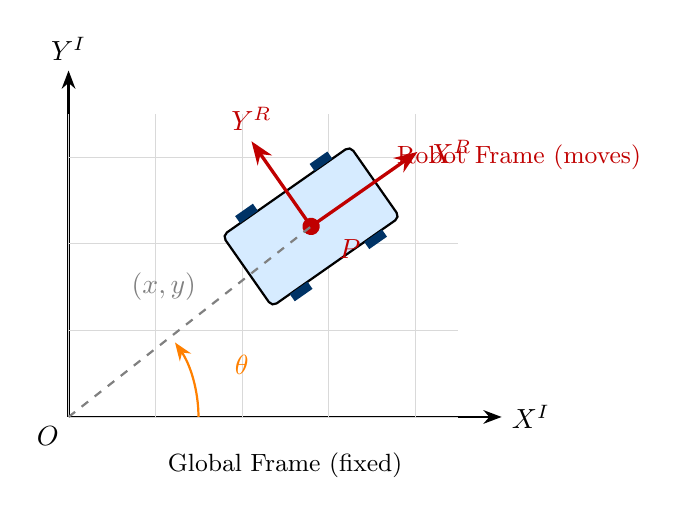
\begin{tikzpicture}[scale=1.1, >=Stealth]
    % Global frame
    \draw[thick, ->] (0,0) -- (5,0) node[right] {$X^I$};
    \draw[thick, ->] (0,0) -- (0,4) node[above] {$Y^I$};
    \node[below left] at (0,0) {$O$};
    
    % Grid (faint)
    \draw[very thin, gray!30] (0,0) grid (4.5,3.5);
    
    % Robot body
    \begin{scope}[shift={(2.8,2.2)}, rotate=35]
        \draw[thick, fill=lightblue!40, rounded corners=2pt] (-0.9,-0.5) rectangle (0.9,0.5);
        % Wheels
        \fill[darkblue] (-0.65,-0.6) rectangle (-0.4,-0.5);
        \fill[darkblue] (0.4,-0.6) rectangle (0.65,-0.5);
        \fill[darkblue] (-0.65,0.5) rectangle (-0.4,0.6);
        \fill[darkblue] (0.4,0.5) rectangle (0.65,0.6);
        % Robot frame
        \draw[very thick, accentred, ->] (0,0) -- (1.5,0) node[right] {$X^R$};
        \draw[very thick, accentred, ->] (0,0) -- (0,1.2) node[above] {$Y^R$};
        \fill[accentred] (0,0) circle (0.1);
        \node[accentred, below right] at (0.15,-0.15) {$P$};
    \end{scope}
    
    % Position vector
    \draw[thick, dashed, gray] (0,0) -- (2.8,2.2);
    \node[gray] at (1.1,1.5) {$(x,y)$};
    
    % Angle theta
    \draw[thick, accentorange, ->] (1.5,0) arc (0:35:1.5);
    \node[accentorange] at (2,0.6) {$\theta$};
    
    % Labels
    \node[below, font=\small] at (2.5,-0.3) {Global Frame (fixed)};
    \node[accentred, font=\small] at (5.2,3) {Robot Frame (moves)};
\end{tikzpicture}
\end{center}

\end{frame}

% -----------------------------------------------------------------------------
\begin{frame}{Global Frame}

\textbf{Global (Inertial) Frame} $(X^I, Y^I)$:

\vspace{0.5cm}

\begin{itemize}
    \item Fixed to the world --- does not move
    
    \vspace{0.3cm}
    
    \item Used to describe:
    \begin{itemize}
        \item Maps and environments
        \item Goal positions
        \item Trajectories
    \end{itemize}
    
    \vspace{0.3cm}
    
    \item Origin $O$ is a fixed reference point
\end{itemize}

\end{frame}

% -----------------------------------------------------------------------------
\begin{frame}{Robot Frame}

\textbf{Robot (Body) Frame} $(X^R, Y^R)$:

\vspace{0.5cm}

\begin{itemize}
    \item Attached to the robot at reference point $P$
    
    \vspace{0.3cm}
    
    \item $P$ is often placed at the center of the wheel axle
    
    \vspace{0.3cm}
    
    \item $X^R$ points forward (heading direction)
    
    \vspace{0.3cm}
    
    \item $Y^R$ points to the left of the robot
    
    \vspace{0.3cm}
    
    \item Moves and rotates with the robot
\end{itemize}

\end{frame}

% -----------------------------------------------------------------------------
\begin{frame}{Robot Pose}

The \textbf{pose} of the robot is defined by three quantities:

\vspace{0.5cm}

\begin{itemize}
    \item $x$: position along global $X^I$ axis
    
    \vspace{0.2cm}
    
    \item $y$: position along global $Y^I$ axis
    
    \vspace{0.2cm}
    
    \item $\theta$: orientation of $X^R$ with respect to $X^I$
\end{itemize}

\vspace{0.5cm}

\begin{block}{Pose Vector}
\[
\vect{\xi}^I = \begin{bmatrix} x \\ y \\ \theta \end{bmatrix}
\]
\end{block}

\end{frame}

% -----------------------------------------------------------------------------
\begin{frame}{Rotation Matrix Between Frames}

The relationship between frames is captured by the \textbf{rotation matrix}:

\vspace{0.5cm}

\begin{block}{Rotation Matrix $R(\theta)$}
\[
R(\theta) = \begin{bmatrix} 
\cos\theta & \sin\theta & 0 \\
-\sin\theta & \cos\theta & 0 \\
0 & 0 & 1
\end{bmatrix}
\]
\end{block}

\vspace{0.5cm}

This matrix transforms vectors from the \textbf{global frame} to the \textbf{robot frame}.

\end{frame}

% -----------------------------------------------------------------------------
\begin{frame}{Rotation Matrix: Properties}

\textbf{Key Properties:}

\vspace{0.5cm}

\begin{itemize}
    \item $R(\theta)^{-1} = R(\theta)^T = R(-\theta)$
    
    \vspace{0.3cm}
    
    \item The matrix is \textbf{orthogonal}: $R^T R = I$
    
    \vspace{0.3cm}
    
    \item $\det(R) = 1$ (proper rotation, no reflection)
    
    \vspace{0.3cm}
    
    \item The third row/column handles $\theta$, which is the same in both frames
\end{itemize}

\end{frame}

% -----------------------------------------------------------------------------
\begin{frame}{Velocity in Different Frames}

Robot velocities can be expressed in either frame:

\vspace{0.5cm}

\textbf{Global frame velocities:}
\[
\dot{\vect{\xi}}^I = \begin{bmatrix} \dot{x} \\ \dot{y} \\ \dot{\theta} \end{bmatrix}
\]

\vspace{0.3cm}

\textbf{Robot frame velocities:}
\[
\dot{\vect{\xi}}^R = \begin{bmatrix} v_x \\ v_y \\ \omega \end{bmatrix}
\]

where $v_x$ = forward, $v_y$ = lateral, $\omega$ = angular velocity.

\end{frame}

% -----------------------------------------------------------------------------
\begin{frame}{Velocity Transformation}

\begin{block}{Velocity Mapping}
\[
\boxed{\dot{\vect{\xi}}^R = R(\theta) \, \dot{\vect{\xi}}^I}
\]
\end{block}

\vspace{0.5cm}

\textbf{Key insight:} This mapping is \textbf{pose-dependent}.

\vspace{0.3cm}

It depends on the current orientation $\theta$ of the robot.

\vspace{0.5cm}

\textbf{Inverse transformation} (robot $\to$ global):
\[
\dot{\vect{\xi}}^I = R(\theta)^{-1} \dot{\vect{\xi}}^R = R(-\theta) \dot{\vect{\xi}}^R
\]

\end{frame}

% -----------------------------------------------------------------------------
\begin{frame}{Example: Robot at $\theta = \pi/2$}

When the robot faces the $Y^I$ direction ($\theta = \pi/2$):

\vspace{0.3cm}

\[
R\left(\frac{\pi}{2}\right) = \begin{bmatrix}
\cos\frac{\pi}{2} & \sin\frac{\pi}{2} & 0 \\[0.1cm]
-\sin\frac{\pi}{2} & \cos\frac{\pi}{2} & 0 \\[0.1cm]
0 & 0 & 1
\end{bmatrix} = \begin{bmatrix}
0 & 1 & 0 \\
-1 & 0 & 0 \\
0 & 0 & 1
\end{bmatrix}
\]

\end{frame}

% -----------------------------------------------------------------------------
\begin{frame}{Example: Velocity Mapping at $\theta = \pi/2$}

\textbf{Velocity mapping:}
\[
\dot{\vect{\xi}}^R = R\left(\frac{\pi}{2}\right) \dot{\vect{\xi}}^I = \begin{bmatrix}
0 & 1 & 0 \\
-1 & 0 & 0 \\
0 & 0 & 1
\end{bmatrix} \begin{bmatrix} \dot{x} \\ \dot{y} \\ \dot{\theta} \end{bmatrix} = \begin{bmatrix} \dot{y} \\ -\dot{x} \\ \dot{\theta} \end{bmatrix}
\]

\vspace{0.5cm}

\textbf{Interpretation:}
\begin{itemize}
    \item Robot's forward velocity: $v_x = \dot{y}$
    \item Robot's lateral velocity: $v_y = -\dot{x}$
    \item Angular velocity: $\omega = \dot{\theta}$ (same in both frames)
\end{itemize}

\end{frame}

% -----------------------------------------------------------------------------
\begin{frame}{Nonholonomic Constraint}

\textbf{Key constraint:} Wheeled robots cannot move sideways.

\vspace{0.5cm}

This means no lateral slip --- the wheels roll, they don't skid sideways.

\vspace{0.5cm}

In the robot frame, this constraint is:

\begin{block}{No Side-Slip Constraint}
\[
\boxed{v_y = 0}
\]
\end{block}

\vspace{0.3cm}

This is called a \textbf{nonholonomic constraint}.

\end{frame}

% -----------------------------------------------------------------------------
\begin{frame}{What is a Nonholonomic Constraint?}

\textbf{Nonholonomic} = restricts \textbf{velocity} but not \textbf{position}.

\vspace{0.5cm}

\begin{itemize}
    \item The robot \textbf{can} reach any position $(x, y)$ and orientation $\theta$
    
    \vspace{0.3cm}
    
    \item The robot \textbf{cannot} move instantaneously sideways
    
    \vspace{0.3cm}
    
    \item It must maneuver (like parallel parking a car)
\end{itemize}

\vspace{0.5cm}

\textbf{Contrast with holonomic:} A holonomic robot (like omni-drive) can move in any direction instantly.

\end{frame}

% -----------------------------------------------------------------------------
\begin{frame}{The Unicycle Model}

With $v_y = 0$, the robot kinematics simplify to:

\vspace{0.5cm}

\begin{block}{Unicycle Kinematic Equations}
\begin{align*}
\dot{x} &= v_x \cos\theta \\[0.2cm]
\dot{y} &= v_x \sin\theta \\[0.2cm]
\dot{\theta} &= \omega
\end{align*}
\end{block}

\vspace{0.3cm}

This is the \textbf{unicycle model} --- a planar rigid body with no lateral motion.

\end{frame}

% -----------------------------------------------------------------------------
\begin{frame}{Unicycle Model: Visualization}

\begin{center}
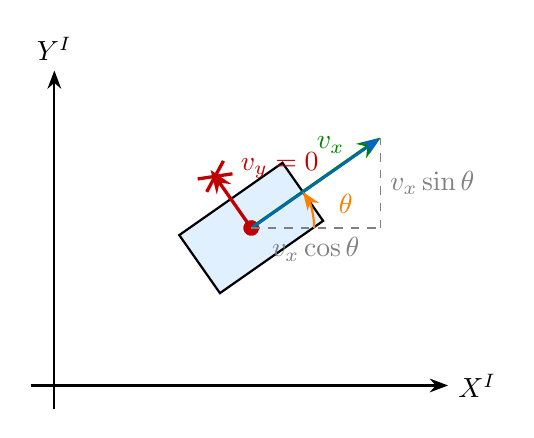
\begin{tikzpicture}[scale=1.0, >=Stealth]
    % Global frame
    \draw[thick, ->] (-0.3,0) -- (5,0) node[right] {$X^I$};
    \draw[thick, ->] (0,-0.3) -- (0,4) node[above] {$Y^I$};
    
    % Robot
    \begin{scope}[shift={(2.5,2)}, rotate=35]
        \draw[thick, fill=lightblue!30] (-0.8,-0.45) rectangle (0.8,0.45);
        \fill[accentred] (0,0) circle (0.1);
        
        % Forward velocity
        \draw[very thick, accentgreen, ->] (0,0) -- (2,0);
        \node[accentgreen, above] at (1.3,0.1) {$v_x$};
        
        % Blocked lateral
        \draw[very thick, accentred, ->] (0,0) -- (0,0.9);
        \draw[very thick, accentred] (-0.2,0.7) -- (0.2,0.9);
        \draw[very thick, accentred] (-0.2,0.9) -- (0.2,0.7);
        \node[accentred, right] at (0.25,0.8) {$v_y = 0$};
    \end{scope}
    
    % Global velocity components
    \draw[thick, brightblue, ->] (2.5,2) -- (4.14,3.14);
    \draw[dashed, gray] (2.5,2) -- (4.14,2) node[midway, below] {$v_x\cos\theta$};
    \draw[dashed, gray] (4.14,2) -- (4.14,3.14) node[midway, right] {$v_x\sin\theta$};
    
    % Angle
    \draw[thick, accentorange, ->] (3.3,2) arc (0:35:0.8);
    \node[accentorange] at (3.7,2.3) {$\theta$};
\end{tikzpicture}
\end{center}

The robot moves in the direction of its heading $\theta$.

\end{frame}

% =============================================================================
% PART 2: DIFFERENTIAL DRIVE
% =============================================================================
\begin{frame}{Differential-Drive Robots}

\begin{center}
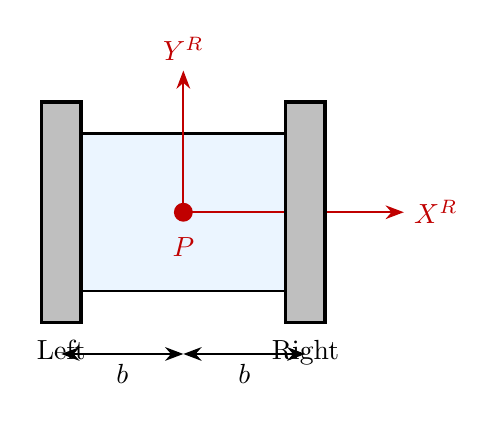
\begin{tikzpicture}[scale=1.0, >=Stealth]
    % Robot body (top view)
    \draw[thick, fill=lightblue!20] (-1.8,-1) rectangle (1.8,1);
    
    % Center point
    \fill[accentred] (0,0) circle (0.12);
    \node[accentred, below] at (0,-0.2) {$P$};
    
    % Robot frame
    \draw[thick, accentred, ->] (0,0) -- (2.8,0) node[right] {$X^R$};
    \draw[thick, accentred, ->] (0,0) -- (0,1.8) node[above] {$Y^R$};
    
    % Left wheel
    \draw[very thick, fill=gray!50] (-1.8,-1.4) rectangle (-1.3,1.4);
    \node[below] at (-1.55,-1.5) {Left};
    
    % Right wheel
    \draw[very thick, fill=gray!50] (1.3,-1.4) rectangle (1.8,1.4);
    \node[below] at (1.55,-1.5) {Right};
    
    % Dimensions
    \draw[thick, <->] (0,-1.8) -- (1.55,-1.8) node[midway, below] {$b$};
    \draw[thick, <->] (-1.55,-1.8) -- (0,-1.8) node[midway, below] {$b$};
\end{tikzpicture}
\end{center}

\end{frame}

% -----------------------------------------------------------------------------
\begin{frame}{Differential-Drive: Parameters}

\textbf{Parameters:}

\vspace{0.5cm}

\begin{itemize}
    \item $r$ = wheel radius
    
    \vspace{0.3cm}
    
    \item $b$ = half the axle length (distance from center to wheel)
    
    \vspace{0.3cm}
    
    \item $\dot{\phi}_1$ = right wheel angular speed (rad/s)
    
    \vspace{0.3cm}
    
    \item $\dot{\phi}_2$ = left wheel angular speed (rad/s)
\end{itemize}

\end{frame}

% -----------------------------------------------------------------------------
\begin{frame}{Differential-Drive: Sign Conventions}

\textbf{Sign conventions:}

\vspace{0.5cm}

\begin{itemize}
    \item Forward motion $(+)$: $v_x > 0$
    
    \vspace{0.3cm}
    
    \item Counter-clockwise yaw $(+)$: $\omega > 0$
    
    \vspace{0.3cm}
    
    \item Right wheel is at position $+b$
    
    \vspace{0.3cm}
    
    \item Left wheel is at position $-b$
\end{itemize}

\vspace{0.5cm}

\textbf{Key relationship:} Each wheel's linear velocity is $v = r \cdot \dot{\phi}$

\end{frame}

% -----------------------------------------------------------------------------
\begin{frame}{Wheel Velocities}

Each wheel's linear velocity combines forward motion and rotation.

\vspace{0.5cm}

\textbf{Right wheel} (at position $+b$):
\[
v_{\text{right}} = v_x + b \cdot \omega
\]

\vspace{0.3cm}

\textbf{Left wheel} (at position $-b$):
\[
v_{\text{left}} = v_x - b \cdot \omega
\]

\end{frame}

% -----------------------------------------------------------------------------
\begin{frame}{Wheel Velocity Equations}

Since linear velocity $v = r\dot{\phi}$:

\vspace{0.5cm}

\begin{block}{Right Wheel}
\[
r\dot{\phi}_1 = v_x + b\omega
\]
\end{block}

\vspace{0.3cm}

\begin{block}{Left Wheel}
\[
r\dot{\phi}_2 = v_x - b\omega
\]
\end{block}

\end{frame}

% -----------------------------------------------------------------------------
\begin{frame}{Physical Interpretation}

\begin{center}
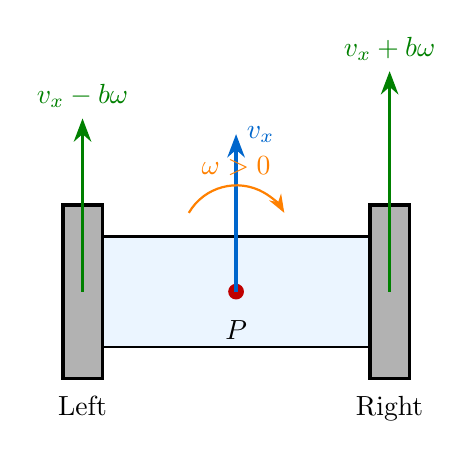
\begin{tikzpicture}[scale=1.0, >=Stealth]
    % Robot body
    \draw[thick, fill=lightblue!20] (-2.2,-0.7) rectangle (2.2,0.7);
    
    % Center
    \fill[accentred] (0,0) circle (0.1);
    \node[below] at (0,-0.25) {$P$};
    
    % Wheels
    \draw[very thick, fill=gray!60] (-2.2,-1.1) rectangle (-1.7,1.1);
    \draw[very thick, fill=gray!60] (1.7,-1.1) rectangle (2.2,1.1);
    
    % Velocity arrows
    \draw[very thick, accentgreen, ->] (-1.95,0) -- (-1.95,2.2) node[above] {$v_x - b\omega$};
    \draw[very thick, accentgreen, ->] (1.95,0) -- (1.95,2.8) node[above] {$v_x + b\omega$};
    
    % Forward velocity at center
    \draw[very thick, brightblue, ->] (0,0) -- (0,2) node[right] {$v_x$};
    
    % Angular velocity
    \draw[thick, accentorange, ->] (-0.6,1) arc (150:30:0.7);
    \node[accentorange] at (0,1.6) {$\omega > 0$};
    
    % Labels
    \node[below] at (-1.95,-1.2) {Left};
    \node[below] at (1.95,-1.2) {Right};
\end{tikzpicture}
\end{center}

\end{frame}

% -----------------------------------------------------------------------------
\begin{frame}{Physical Interpretation: Cases}

\textbf{When $\omega > 0$ (turning left):}
\begin{itemize}
    \item Right wheel moves faster than left wheel
\end{itemize}

\vspace{0.4cm}

\textbf{When $\omega = 0$ (going straight):}
\begin{itemize}
    \item Both wheels have the same speed
\end{itemize}

\vspace{0.4cm}

\textbf{When $v_x = 0$ and $\omega \neq 0$:}
\begin{itemize}
    \item Robot spins in place
\end{itemize}

\end{frame}

% -----------------------------------------------------------------------------
\begin{frame}{Solving for Body Velocities}

Add the two wheel equations:
\[
r\dot{\phi}_1 + r\dot{\phi}_2 = 2v_x
\]

\vspace{0.2cm}

\begin{block}{Forward Velocity}
\[
v_x = \frac{r}{2}(\dot{\phi}_1 + \dot{\phi}_2)
\]
\end{block}

\vspace{0.3cm}

Subtract the two wheel equations:
\[
r\dot{\phi}_1 - r\dot{\phi}_2 = 2b\omega
\]

\vspace{0.2cm}

\begin{block}{Angular Velocity}
\[
\omega = \frac{r}{2b}(\dot{\phi}_1 - \dot{\phi}_2)
\]
\end{block}

\end{frame}

% -----------------------------------------------------------------------------
\begin{frame}{Jacobian Form}

\begin{block}{Jacobian Mapping (Robot Frame)}
\[
\begin{bmatrix} v_x \\ v_y \\ \omega \end{bmatrix} = 
\underbrace{\begin{bmatrix} 
\frac{r}{2} & \frac{r}{2} \\[0.2cm]
0 & 0 \\[0.2cm]
\frac{r}{2b} & -\frac{r}{2b}
\end{bmatrix}}_{J^R}
\begin{bmatrix} \dot{\phi}_1 \\ \dot{\phi}_2 \end{bmatrix}
\]
\end{block}

\vspace{0.5cm}

The Jacobian $J^R$ maps wheel angular velocities to body velocities.

\vspace{0.3cm}

Note: $v_y = 0$ always (nonholonomic constraint).

\end{frame}

% -----------------------------------------------------------------------------
\begin{frame}{Forward Kinematics in Global Frame}

To navigate, we need motion in \textbf{global coordinates}.

\vspace{0.5cm}

Transform from robot frame to global frame:

\vspace{0.3cm}

\begin{block}{Global Frame Kinematics}
\[
\dot{\vect{\xi}}^I = R(-\theta) \begin{bmatrix} v_x \\ 0 \\ \omega \end{bmatrix} = \begin{bmatrix} v_x \cos\theta \\ v_x \sin\theta \\ \omega \end{bmatrix}
\]
\end{block}

\end{frame}

% -----------------------------------------------------------------------------
\begin{frame}{Forward Kinematics: Expanded}

\textbf{Expanded form:}

\vspace{0.5cm}

\begin{align*}
\dot{x} &= \frac{r}{2}(\dot{\phi}_1 + \dot{\phi}_2) \cos\theta \\[0.3cm]
\dot{y} &= \frac{r}{2}(\dot{\phi}_1 + \dot{\phi}_2) \sin\theta \\[0.3cm]
\dot{\theta} &= \frac{r}{2b}(\dot{\phi}_1 - \dot{\phi}_2)
\end{align*}

\vspace{0.3cm}

These equations describe how wheel speeds produce robot motion.

\end{frame}

% =============================================================================
% PART 3: BICYCLE MODEL
% =============================================================================
\begin{frame}{Why Do We Need Dynamics?}

\textbf{Kinematics} only explains how velocity inputs produce motion.

\vspace{0.5cm}

For car-like robots (Ackermann steering):
\begin{itemize}
    \item Forces and inertia matter
    \item Need to model turning, drifting, braking
\end{itemize}

\vspace{0.5cm}

\textbf{Newton's Laws:}
\[
\sum \vect{F} = m\vect{a}, \quad \sum M = I\dot{\omega}
\]

\end{frame}

% -----------------------------------------------------------------------------
\begin{frame}{The Bicycle Model}

\begin{columns}
\begin{column}{0.5\textwidth}
\textbf{Simplification:}
\begin{itemize}
    \item 4-wheel vehicle $\to$ 2-wheel equivalent
    \item Front wheel can steer (angle $\delta$)
    \item Rear wheel is fixed
    \item Reference: Center of Mass (COM)
\end{itemize}
\end{column}
\begin{column}{0.5\textwidth}
\centering
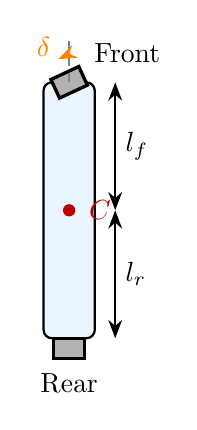
\begin{tikzpicture}[scale=0.65, >=Stealth]
    % Vehicle body
    \draw[thick, fill=lightblue!20, rounded corners=3pt] (-0.5,-2.5) rectangle (0.5,2.5);
    
    % COM
    \fill[accentred] (0,0) circle (0.12);
    \node[accentred, right] at (0.2,0) {$C$};
    
    % Rear wheel
    \draw[very thick, fill=gray!60] (-0.3,-2.5) rectangle (0.3,-2.9);
    \node[below] at (0,-3) {Rear};
    
    % Front wheel (steered)
    \begin{scope}[shift={(0,2.5)}, rotate=25]
        \draw[very thick, fill=gray!60] (-0.3,-0.2) rectangle (0.3,0.2);
    \end{scope}
    \node[above right] at (0.3,2.7) {Front};
    
    % Steering angle
    \draw[thick, gray, dashed] (0,2.5) -- (0,3.3);
    \draw[thick, accentorange, ->] (0,3) arc (90:115:0.5);
    \node[accentorange] at (-0.5,3.2) {$\delta$};
    
    % Distances
    \draw[thick, <->] (0.9,0) -- (0.9,2.5) node[midway, right] {$l_f$};
    \draw[thick, <->] (0.9,0) -- (0.9,-2.5) node[midway, right] {$l_r$};
\end{tikzpicture}
\end{column}
\end{columns}

\end{frame}

% -----------------------------------------------------------------------------
\begin{frame}{Bicycle Model: Parameters}

\textbf{Geometric parameters:}
\begin{itemize}
    \item $l_f$: distance from COM to front axle
    \item $l_r$: distance from COM to rear axle
    \item $\delta$: steering angle of front wheel
\end{itemize}

\vspace{0.5cm}

\textbf{Velocities at COM:}
\begin{itemize}
    \item $V_x$: longitudinal velocity
    \item $V_y$: lateral velocity
    \item $\omega$: yaw rate
\end{itemize}

\end{frame}

% -----------------------------------------------------------------------------
\begin{frame}{Forces on the Vehicle}

\begin{columns}
\begin{column}{0.5\textwidth}
\textbf{Forces:}
\begin{itemize}
    \item $F_{xf}, F_{yf}$: forces at front wheel
    \item $F_{xr}, F_{yr}$: forces at rear wheel
\end{itemize}

\vspace{0.5cm}

\textbf{Governing principle:}
\[
\sum \vect{F} = m\vect{a}
\]
\[
\sum M = I\dot{\omega}
\]
\end{column}
\begin{column}{0.5\textwidth}
\centering
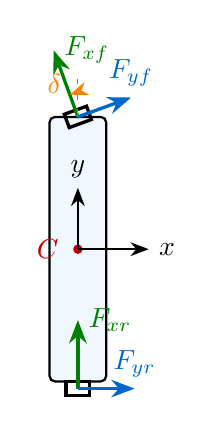
\begin{tikzpicture}[scale=0.6, >=Stealth]
    % Vehicle body
    \draw[thick, fill=lightblue!15, rounded corners=2pt] (-0.6,-2.8) rectangle (0.6,2.8);
    
    % COM
    \fill[accentred] (0,0) circle (0.1);
    \node[accentred, left] at (-0.2,0) {$C$};
    
    % Body frame at COM
    \draw[thick, ->] (0,0) -- (1.5,0) node[right] {$x$};
    \draw[thick, ->] (0,0) -- (0,1.3) node[above] {$y$};
    
    % Rear wheel and forces
    \draw[very thick] (-0.25,-2.8) rectangle (0.25,-3.1);
    \draw[very thick, accentgreen, ->] (0,-2.95) -- (0,-1.5) node[right] {$F_{xr}$};
    \draw[very thick, brightblue, ->] (0,-2.95) -- (1.2,-2.95) node[above] {$F_{yr}$};
    
    % Front wheel (steered) and forces
    \begin{scope}[shift={(0,2.8)}, rotate=20]
        \draw[very thick] (-0.25,-0.15) rectangle (0.25,0.15);
        \draw[very thick, accentgreen, ->] (0,0) -- (0,1.5) node[right] {$F_{xf}$};
        \draw[very thick, brightblue, ->] (0,0) -- (1.2,0) node[above] {$F_{yf}$};
    \end{scope}
    
    % Steering angle
    \draw[dashed, gray] (0,2.8) -- (0,3.6);
    \draw[thick, accentorange, ->] (0,3.3) arc (90:110:0.5);
    \node[accentorange] at (-0.5,3.5) {$\delta$};
\end{tikzpicture}
\end{column}
\end{columns}

\end{frame}

% -----------------------------------------------------------------------------
\begin{frame}{Equations of Motion: Longitudinal}

Applying Newton's laws in the body frame:

\vspace{0.5cm}

\textbf{Longitudinal ($x$-axis):}

\begin{block}{}
\[
m\dot{V}_x - mV_y\omega = F_{xf}\cos\delta - F_{yf}\sin\delta + F_{xr}
\]
\end{block}

\vspace{0.5cm}

The term $mV_y\omega$ is a \textbf{Coriolis effect} from the rotating frame.

\end{frame}

% -----------------------------------------------------------------------------
\begin{frame}{Equations of Motion: Lateral}

\textbf{Lateral ($y$-axis):}

\begin{block}{}
\[
m\dot{V}_y + mV_x\omega = F_{yf}\cos\delta + F_{xf}\sin\delta + F_{yr}
\]
\end{block}

\vspace{0.5cm}

The term $mV_x\omega$ is also a \textbf{Coriolis/centrifugal effect}.

\end{frame}

% -----------------------------------------------------------------------------
\begin{frame}{Equations of Motion: Yaw}

\textbf{Yaw (rotation about $z$-axis):}

\begin{block}{}
\[
I_{zz}\dot{\omega} = l_f(F_{yf}\cos\delta + F_{xf}\sin\delta) - l_r F_{yr}
\]
\end{block}

\vspace{0.5cm}

This describes how torques from tire forces create yaw acceleration.

\end{frame}

% -----------------------------------------------------------------------------
\begin{frame}{Matrix Representation: Mass Matrix}

Define state vector: $\vect{q} = [V_x, V_y, \omega]^T$

\vspace{0.5cm}

\textbf{Mass/Inertia Matrix:}
\[
M = \begin{bmatrix} m & 0 & 0 \\ 0 & m & 0 \\ 0 & 0 & I_{zz} \end{bmatrix}
\]

\end{frame}

% -----------------------------------------------------------------------------
\begin{frame}{Matrix Representation: Coriolis Matrix}

\textbf{Coriolis/Centrifugal terms:}
\[
C\dot{\vect{q}} = \begin{bmatrix} -mV_y\omega \\ mV_x\omega \\ 0 \end{bmatrix}
\]

\vspace{0.5cm}

This can be written as:
\[
C = \begin{bmatrix} 0 & -m\omega & 0 \\ m\omega & 0 & 0 \\ 0 & 0 & 0 \end{bmatrix}
\]

\end{frame}

% -----------------------------------------------------------------------------
\begin{frame}{Compact Dynamic Model}

\begin{block}{Vehicle Dynamics}
\[
\boxed{M\ddot{\vect{q}} + C\dot{\vect{q}} + G = B_y F_y + B_x F_x}
\]
\end{block}

\vspace{0.5cm}

where:
\begin{itemize}
    \item $M$: mass/inertia matrix
    \item $C$: Coriolis matrix
    \item $G = 0$ on flat ground
    \item $B_y, B_x$: input matrices for tire forces
\end{itemize}

\end{frame}

% -----------------------------------------------------------------------------
\begin{frame}{Input Matrices}

\textbf{Lateral force input:}
\[
B_y = \begin{bmatrix} -\sin\delta & 0 \\ \cos\delta & 1 \\ l_f\cos\delta & -l_r \end{bmatrix}, \quad F_y = \begin{bmatrix} F_{yf} \\ F_{yr} \end{bmatrix}
\]

\vspace{0.5cm}

\textbf{Longitudinal force input:}
\[
B_x = \begin{bmatrix} \cos\delta & 1 \\ \sin\delta & 0 \\ l_f\sin\delta & 0 \end{bmatrix}, \quad F_x = \begin{bmatrix} F_{xf} \\ F_{xr} \end{bmatrix}
\]

\end{frame}

% -----------------------------------------------------------------------------
\begin{frame}{Applications of Bicycle Model}

This model is the foundation for:

\vspace{0.5cm}

\begin{itemize}
    \item Vehicle stability control
    
    \vspace{0.3cm}
    
    \item Yaw stability and skid avoidance
    
    \vspace{0.3cm}
    
    \item Path tracking and trajectory control
    
    \vspace{0.3cm}
    
    \item Autonomous vehicle motion planning
\end{itemize}

\end{frame}

% =============================================================================
% PART 4: OMNI-DRIVE
% =============================================================================
\begin{frame}{Omni-Directional Robots}

\textbf{Why omni-drive?}

\vspace{0.5cm}

\begin{itemize}
    \item 3 omni-wheels placed 120° apart
    
    \vspace{0.3cm}
    
    \item Full \textbf{3-DOF control}: $(x, y, \theta)$
    
    \vspace{0.3cm}
    
    \item Robot can move in \textbf{any direction} instantly
    
    \vspace{0.3cm}
    
    \item Can rotate \textbf{without reorientation}
\end{itemize}

\end{frame}

% -----------------------------------------------------------------------------
\begin{frame}{Holonomic vs Nonholonomic}

\textbf{Holonomic system:}
\begin{itemize}
    \item 3 actuators $\leftrightarrow$ 3 DOF
    \item No velocity constraints
    \item Can move sideways instantly
\end{itemize}

\vspace{0.5cm}

\textbf{Contrast with differential drive:}
\begin{itemize}
    \item Differential drive has constraint $v_y = 0$
    \item Cannot move sideways without rotating
\end{itemize}

\end{frame}

% -----------------------------------------------------------------------------
\begin{frame}{Omni-Drive: Geometry}

\begin{center}
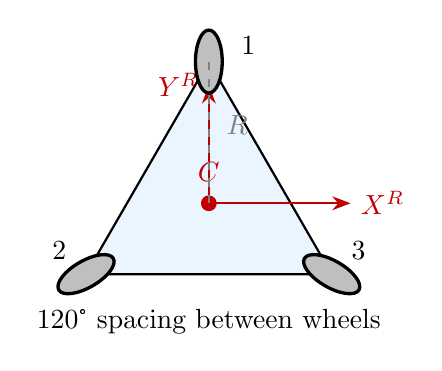
\begin{tikzpicture}[scale=1.0, >=Stealth]
    % Robot body (triangle)
    \draw[thick, fill=lightblue!20] (0,1.8) -- (-1.56,-0.9) -- (1.56,-0.9) -- cycle;
    
    % Center
    \fill[accentred] (0,0) circle (0.1);
    \node[accentred] at (0,0.4) {$C$};
    
    % Robot frame
    \draw[thick, accentred, ->] (0,0) -- (1.8,0) node[right] {$X^R$};
    \draw[thick, accentred, ->] (0,0) -- (0,1.5) node[left] {$Y^R$};
    
    % Wheels
    \draw[very thick, fill=gray!50, rotate around={-90:(0,1.8)}] (0,1.8) ellipse (0.4 and 0.17);
    \node at (0.5,2) {1};
    
    \draw[very thick, fill=gray!50, rotate around={30:(-1.56,-0.9)}] (-1.56,-0.9) ellipse (0.4 and 0.17);
    \node at (-1.9,-0.6) {2};
    
    \draw[very thick, fill=gray!50, rotate around={150:(1.56,-0.9)}] (1.56,-0.9) ellipse (0.4 and 0.17);
    \node at (1.9,-0.6) {3};
    
    % Radius
    \draw[thick, dashed, gray] (0,0) -- (0,1.8);
    \node[gray, right] at (0.1,1) {$R$};
    
    \node at (0,-1.5) {120° spacing between wheels};
\end{tikzpicture}
\end{center}

\end{frame}

% -----------------------------------------------------------------------------
\begin{frame}{Omni-Drive: Parameters}

\textbf{Robot frame:} $(x, y, \theta)$ at center of mass

\vspace{0.3cm}

\textbf{Global frame:} $(X, Y)$ fixed to world

\vspace{0.5cm}

\textbf{Wheel positions:}
\begin{itemize}
    \item Equally spaced at angles $\alpha_1, \alpha_2, \alpha_3$
    \item Each wheel at radius $R$ from center
    \item Individual wheel radius: $r$
\end{itemize}

\vspace{0.5cm}

\textbf{Typical:} $\alpha_1 = 90°$, $\alpha_2 = 210°$, $\alpha_3 = 330°$

\end{frame}

% -----------------------------------------------------------------------------
\begin{frame}{Omni-Drive: Kinematic Mapping}

For wheel $i$ at angle $\alpha_i$:

\begin{block}{Wheel Velocity}
\[
r\dot{\phi}_i = -v_x \sin\alpha_i + v_y \cos\alpha_i + R\omega
\]
\end{block}

\vspace{0.5cm}

\textbf{Matrix form:}
\[
r\begin{bmatrix} \dot{\phi}_1 \\ \dot{\phi}_2 \\ \dot{\phi}_3 \end{bmatrix} = 
\begin{bmatrix} 
-\sin\alpha_1 & \cos\alpha_1 & R \\
-\sin\alpha_2 & \cos\alpha_2 & R \\
-\sin\alpha_3 & \cos\alpha_3 & R
\end{bmatrix}
\begin{bmatrix} v_x \\ v_y \\ \omega \end{bmatrix}
\]

\end{frame}

% -----------------------------------------------------------------------------
\begin{frame}{Omni-Drive: Force Balance}

Apply Newton's laws: $\sum \vect{F} = m\vect{a}$

\vspace{0.5cm}

\textbf{X-direction:}
\[
F_1 \cos\alpha_1 + F_2 \cos\alpha_2 + F_3 \cos\alpha_3 = m\ddot{x}
\]

\vspace{0.3cm}

\textbf{Y-direction:}
\[
F_1 \sin\alpha_1 + F_2 \sin\alpha_2 + F_3 \sin\alpha_3 = m\ddot{y}
\]

\vspace{0.3cm}

\textbf{Rotation:}
\[
R(F_1 + F_2 + F_3) = I_{zz}\ddot{\theta}
\]

\end{frame}

% -----------------------------------------------------------------------------
\begin{frame}{Omni-Drive: Matrix Form}

\begin{block}{Compact Form}
\[
M\ddot{\vect{\xi}} = B\vect{F}
\]
\end{block}

\vspace{0.3cm}

\textbf{Mass matrix:}
\[
M = \begin{bmatrix} m & 0 & 0 \\ 0 & m & 0 \\ 0 & 0 & I_{zz} \end{bmatrix}
\]

\vspace{0.3cm}

\textbf{Input matrix:}
\[
B = \begin{bmatrix}
\cos\alpha_1 & \cos\alpha_2 & \cos\alpha_3 \\
\sin\alpha_1 & \sin\alpha_2 & \sin\alpha_3 \\
R & R & R
\end{bmatrix}
\]

\end{frame}

% -----------------------------------------------------------------------------
\begin{frame}{Properties of the Input Matrix}

\textbf{Key property:} $\det(B) \neq 0$

\vspace{0.5cm}

Therefore:
\begin{itemize}
    \item $B^{-1}$ exists
    
    \vspace{0.3cm}
    
    \item Forces and accelerations are \textbf{uniquely related}
    
    \vspace{0.3cm}
    
    \item Full controllability in all 3 DOF
\end{itemize}

\end{frame}

% =============================================================================
% PART 5: LAGRANGIAN DYNAMICS
% =============================================================================
\begin{frame}{Introduction to Lagrangian Dynamics}

\textbf{Goal:} Derive dynamic models using energy methods.

\vspace{0.5cm}

\textbf{Generalized coordinates:}
\[
\vect{q} = \begin{bmatrix} x \\ y \\ \theta \end{bmatrix}, \quad
\dot{\vect{q}} = \begin{bmatrix} \dot{x} \\ \dot{y} \\ \dot{\theta} \end{bmatrix}
\]

\vspace{0.5cm}

\textbf{Lagrangian:}
\[
L = K - V
\]

where $K$ = kinetic energy, $V$ = potential energy.

\end{frame}

% -----------------------------------------------------------------------------
\begin{frame}{Lagrangian for Planar Robots}

For planar mobile robots on flat ground:

\vspace{0.5cm}

\begin{itemize}
    \item Potential energy: $V = 0$ (no gravity in plane)
    
    \vspace{0.3cm}
    
    \item Lagrangian simplifies to: $L = K$
\end{itemize}

\vspace{0.5cm}

\begin{block}{Euler-Lagrange Equation}
\[
\frac{d}{dt}\left(\frac{\partial L}{\partial \dot{q}_i}\right) - \frac{\partial L}{\partial q_i} = F_i
\]
\end{block}

where $F_i$ are the generalized forces.

\end{frame}

% -----------------------------------------------------------------------------
\begin{frame}{Kinetic Energy}

\textbf{Translational:}
\[
K_t = \frac{1}{2}m(v_x^2 + v_y^2) = \frac{1}{2}m(\dot{x}^2 + \dot{y}^2)
\]

\vspace{0.3cm}

\textbf{Rotational:}
\[
K_r = \frac{1}{2}I_{zz}\omega^2 = \frac{1}{2}I_{zz}\dot{\theta}^2
\]

\vspace{0.3cm}

\textbf{Total:}
\[
K = \frac{1}{2}m(\dot{x}^2 + \dot{y}^2) + \frac{1}{2}I_{zz}\dot{\theta}^2
\]

\end{frame}

% -----------------------------------------------------------------------------
\begin{frame}{The Lagrangian}

\textbf{Lagrangian} (with $V = 0$):
\[
L = K = \frac{1}{2}m(\dot{x}^2 + \dot{y}^2) + \frac{1}{2}I_{zz}\dot{\theta}^2
\]

\vspace{0.5cm}

\textbf{Partial derivatives:}
\begin{align*}
\frac{\partial L}{\partial \dot{x}} &= m\dot{x}, \quad \frac{\partial L}{\partial x} = 0 \\[0.2cm]
\frac{\partial L}{\partial \dot{y}} &= m\dot{y}, \quad \frac{\partial L}{\partial y} = 0 \\[0.2cm]
\frac{\partial L}{\partial \dot{\theta}} &= I_{zz}\dot{\theta}, \quad \frac{\partial L}{\partial \theta} = 0
\end{align*}

\end{frame}

% -----------------------------------------------------------------------------
\begin{frame}{Equations of Motion from Lagrangian}

Applying Euler-Lagrange:

\vspace{0.3cm}

\textbf{For $x$:}
\[
\frac{d}{dt}(m\dot{x}) = F_x \quad \Rightarrow \quad m\ddot{x} = F_x
\]

\vspace{0.2cm}

\textbf{For $y$:}
\[
\frac{d}{dt}(m\dot{y}) = F_y \quad \Rightarrow \quad m\ddot{y} = F_y
\]

\vspace{0.2cm}

\textbf{For $\theta$:}
\[
\frac{d}{dt}(I_{zz}\dot{\theta}) = \tau \quad \Rightarrow \quad I_{zz}\ddot{\theta} = \tau
\]

\end{frame}

% -----------------------------------------------------------------------------
\begin{frame}{Matrix Form from Lagrangian}

\begin{block}{Equations of Motion}
\[
\begin{bmatrix} m & 0 & 0 \\ 0 & m & 0 \\ 0 & 0 & I_{zz} \end{bmatrix}
\begin{bmatrix} \ddot{x} \\ \ddot{y} \\ \ddot{\theta} \end{bmatrix} = 
\begin{bmatrix} F_x \\ F_y \\ \tau \end{bmatrix}
\]
\end{block}

\vspace{0.5cm}

The generalized forces $(F_x, F_y, \tau)$ come from wheel forces mapped to the global frame.

\end{frame}

% =============================================================================
% SUMMARY
% =============================================================================
\begin{frame}{Summary: Reference Frames}

\begin{itemize}
    \item Global (inertial) vs.\ Robot (body) frames
    
    \vspace{0.3cm}
    
    \item Rotation matrix $R(\theta)$ transforms between frames
    
    \vspace{0.3cm}
    
    \item Velocity mapping: $\dot{\vect{\xi}}^R = R(\theta)\dot{\vect{\xi}}^I$
\end{itemize}

\end{frame}

% -----------------------------------------------------------------------------
\begin{frame}{Summary: Differential Drive}

\begin{itemize}
    \item Nonholonomic constraint: $v_y = 0$
    
    \vspace{0.3cm}
    
    \item Unicycle model: $\dot{x} = v_x\cos\theta$, $\dot{y} = v_x\sin\theta$
    
    \vspace{0.3cm}
    
    \item Jacobian maps wheel velocities to body velocities
    
    \vspace{0.3cm}
    
    \item $v_x = \frac{r}{2}(\dot{\phi}_1 + \dot{\phi}_2)$, $\omega = \frac{r}{2b}(\dot{\phi}_1 - \dot{\phi}_2)$
\end{itemize}

\end{frame}

% -----------------------------------------------------------------------------
\begin{frame}{Summary: Bicycle Model}

\begin{itemize}
    \item Dynamics include forces, inertia, Coriolis terms
    
    \vspace{0.3cm}
    
    \item Compact form: $M\ddot{\vect{q}} + C\dot{\vect{q}} = B_y F_y + B_x F_x$
    
    \vspace{0.3cm}
    
    \item Foundation for vehicle control and stability
\end{itemize}

\end{frame}

% -----------------------------------------------------------------------------
\begin{frame}{Summary: Omni-Drive \& Lagrangian}

\textbf{Omni-Drive:}
\begin{itemize}
    \item Holonomic: full 3-DOF control
    \item $M\ddot{\vect{\xi}} = B\vect{F}$
\end{itemize}

\vspace{0.5cm}

\textbf{Lagrangian Dynamics:}
\begin{itemize}
    \item Energy-based derivation: $L = K - V$
    \item Euler-Lagrange equations give equations of motion
\end{itemize}

\end{frame}

% -----------------------------------------------------------------------------
\begin{frame}{}
\begin{center}
\vspace{2cm}

{\Large \textbf{End of Lecture 2}}

\vspace{1.5cm}

{\large Vehicle Kinematics \& Equations of Motion}

\vspace{2cm}

Questions?
\end{center}
\end{frame}

\end{document}
